% !TeX program = xelatex
\documentclass[a4paper,10pt]{article}

% ============================================================================
% សន្លឹកកិច្ចការសិស្ស ស-ខ្មៅ (No-LCD Student Fill-In Worksheet - Grade 8 Lesson 14.1)
% ត្រូវគ្នា ១០០% នឹង LS_Plan_AREA1.tex | ២ ទំព័រ A4 ពេញ (>=90% Page Utilization)
% ============================================================================
\usepackage[a4paper, left=1.0cm, right=1.0cm, top=0.80cm, bottom=1.00cm, footskip=0.50cm]{geometry}
\usepackage{amsmath, amssymb}
\usepackage{unicode-math}
\usepackage{fontspec}
\usepackage{array, colortbl}
\usepackage[table]{xcolor}
\usepackage{enumitem}
\usepackage{pifont}
\usepackage{fancyhdr}
\usepackage{lastpage}
\usepackage{tikz}
\usepackage[most]{tcolorbox}
\usetikzlibrary{calc, arrows.meta, angles, quotes, decorations.markings, positioning, babel}

\makeatletter
\let\@expl@@@mark@update@singlecol@structures@@\relax
\makeatother

% ============================================================================
% ការកំណត់ពុម្ពអក្សរផ្លូវការ (Cross-Platform Windows + Cloud fonts/)
% ============================================================================
\providecommand{\NGSFindFonts}{%
  \IfFileExists{C:/Windows/Fonts/cambria.ttc}{%
    \def\NGSSysPath{C:/Windows/Fonts/}%
    \def\NGSUserPath{C:/Users/KIT/AppData/Local/Microsoft/Windows/Fonts/}%
  }{%
    \IfFileExists{./fonts/KhmerOSsiemreap.ttf}{\def\NGSSysPath{./fonts/}\def\NGSUserPath{./fonts/}}{%
    \IfFileExists{../fonts/KhmerOSsiemreap.ttf}{\def\NGSSysPath{../fonts/}\def\NGSUserPath{../fonts/}}{%
    \IfFileExists{../../fonts/KhmerOSsiemreap.ttf}{\def\NGSSysPath{../../fonts/}\def\NGSUserPath{../../fonts/}}{%
    \IfFileExists{../../../fonts/KhmerOSsiemreap.ttf}{\def\NGSSysPath{../../../fonts/}\def\NGSUserPath{../../../fonts/}}{%
    \IfFileExists{../../../../fonts/KhmerOSsiemreap.ttf}{\def\NGSSysPath{../../../../fonts/}\def\NGSUserPath{../../../../fonts/}}{%
    \IfFileExists{../../../../../fonts/KhmerOSsiemreap.ttf}{\def\NGSSysPath{../../../../../fonts/}\def\NGSUserPath{../../../../../fonts/}}{%
    \IfFileExists{../../../../../../fonts/KhmerOSsiemreap.ttf}{\def\NGSSysPath{../../../../../../fonts/}\def\NGSUserPath{../../../../../../fonts/}}{%
      \def\NGSSysPath{../../../../../../../fonts/}\def\NGSUserPath{../../../../../../../fonts/}%
    }}}}}}}%
  }%
}
\NGSFindFonts

\setmathfont[Path={\NGSSysPath}, FontIndex=1, Scale=1.02]{cambria.ttc}
\defaultfontfeatures{Ligatures=TeX}

\setmainfont[
  Path={\NGSUserPath},
  Extension=.ttf,
  Script=Khmer,
  BoldFont={KhmerOSsiemreap},
  BoldFeatures={FakeBold=1.8},
  ItalicFont={KhmerOSsiemreap},
  ItalicFeatures={FakeSlant=0.25},
  BoldItalicFont={KhmerOSsiemreap},
  BoldItalicFeatures={FakeBold=1.8, FakeSlant=0.25}
]{KhmerOSsiemreap}

\newfontfamily\muol[Path={\NGSUserPath}, Extension=.ttf, Script=Khmer]{KhmerOSmuollight}
\newfontfamily\TimesEn[Path={\NGSSysPath}, Extension=.ttf, BoldFont={timesbd}, ItalicFont={timesi}, BoldItalicFont={timesbi}]{times}
\newfontfamily\CalibriFont[Path={\NGSSysPath}, Extension=.ttf]{calibri}

\XeTeXlinebreaklocale "km"
\XeTeXlinebreakskip = 0pt plus 1pt minus 0.1pt

% Strict B&W Print Palette
\definecolor{panelgray}{gray}{0.93}
\definecolor{headgray}{gray}{0.85}

\pagestyle{fancy}
\fancyhf{}
\renewcommand{\headrulewidth}{0pt}
\fancyfoot[L]{\fontsize{8.0pt}{10pt}\selectfont អនុវិទ្យាល័យព្រះក្រសាំង \en{|} គណិតវិទ្យា ថ្នាក់ទី៨ \en{|} មេរៀនទី១៤ (១៤.១) ផ្ទៃក្រឡាប្រលេឡូក្រាម និងត្រីកោណ}
\fancyfoot[R]{\fontsize{8.2pt}{10pt}\selectfont ទំព័រ \en{\thepage\ / \pageref{LastPage}}}

\setlength{\parindent}{0pt}
\setlength{\parskip}{0pt}
\setlength{\tabcolsep}{4pt}

\newcommand{\en}[1]{{\TimesEn #1}}
\newcommand{\enbf}[1]{{\TimesEn\bfseries #1}}
\newcommand{\unit}[1]{\,\text{\en{#1}}}
\newcommand{\cnum}[1]{\mbox{\fontsize{10pt}{12pt}\selectfont\ding{\numexpr181+#1\relax}}}
\newcommand{\chkbox}{\tikz[baseline=-0.18ex]\draw[black, line width=0.85pt] (0,0) rectangle (0.26cm,0.26cm);}
\newcommand{\blank}[1]{\makebox[#1]{\dotfill}}
\newcommand{\tri}[1]{\ensuremath{\triangle #1}}
\newcommand{\ang}[1]{\ensuremath{\angle #1}}
\newcommand{\cg}{\ensuremath{\cong}}

\newcommand{\rightbox}[4][0.22cm]{%
  \draw[black, line width=0.8pt]
    ($(#3)!#1!(#2)$) -- ($($(#3)!#1!(#2)$)+($(#3)!#1!(#4)$)-(#3)$) -- ($(#3)!#1!(#4)$);
}

\newcommand{\secbar}[2]{%
  \begin{tcolorbox}[
    enhanced, sharp corners, colback=headgray, colframe=black,
    boxrule=1.0pt, boxsep=1pt, top=2.5pt, bottom=2.5pt, left=6pt, right=6pt,
    before skip=4pt, after skip=3.5pt
  ]
    {\muol\fontsize{9.2pt}{13.5pt}\selectfont #1}\hfill{\fontsize{8.3pt}{11.5pt}\selectfont\textbf{#2}}
  \end{tcolorbox}%
}

\begin{document}
\fontsize{9.4pt}{13.8pt}\selectfont

% ==================== ក្បាលសន្លឹកកិច្ចការ (ទំព័រទី ១) ====================
\begin{tcolorbox}[
  enhanced, sharp corners, colback=white, colframe=black,
  boxrule=1.1pt, boxsep=2pt, top=4pt, bottom=4pt, left=6pt, right=6pt, after skip=4pt
]
  \begin{minipage}[c]{11.5cm}
    {\muol\fontsize{10.2pt}{15pt}\selectfont សន្លឹកកិច្ចការសិស្ស — មេរៀនទី១៤ ៖ ផ្ទៃក្រឡាពហុកោណ}\\[2pt]
    \textbf{ចំណុចទី ១ ៖ ផ្ទៃក្រឡាប្រលេឡូក្រាម និងវិបាកផ្ទៃក្រឡាត្រីកោណ} (សៀវភៅគោល ទំ.១៨៧--១៩០)
  \end{minipage}\hfill
  \begin{minipage}[c]{6.8cm}
    ឈ្មោះសិស្ស៖ \blank{4.5cm}\\[2pt]
    ថ្នាក់ទី៨៖ \blank{1.4cm}\hspace{0.2cm} ដៃគូទី៖ \blank{2.2cm}
  \end{minipage}
\end{tcolorbox}

% ==================== ផ្នែកទី ១ ៖ E1 - ENGAGE ====================
\secbar{ផ្នែកទី ១ ៖ បេសកកម្មភ្ជាប់បញ្ហា (\enbf{E1}) — ដីស្រែពីរក្បែរប្រឡាយទឹក}{\en{3} នាទី (ទស្សន៍ទាយមុនរៀន)}

\begin{tcolorbox}[
  enhanced, sharp corners, colback=panelgray, colframe=black,
  boxrule=0.9pt, boxsep=2pt, top=3pt, bottom=3pt, left=6pt, right=6pt, after skip=4pt
]
  \begin{minipage}[c]{10.2cm}
    កសិករពីរនាក់មានដីស្រែជាប់ប្រឡាយទឹកដូចរូបខាងស្ដាំ៖
    \begin{itemize}[leftmargin=1.3em, itemsep=1pt, topsep=2pt]
      \item \textbf{ស្រែទី១ (ចតុកោណកែង)៖} បាត $8\unit{m}$ និងទទឹងកែង $3\unit{m}$ មានផ្ទៃ $S_1 = 8\times 3 = 24\unit{m}^2$។
      \item \textbf{ស្រែទី២ (ប្រលេឡូក្រាមទ្រេត)៖} បាត $8\unit{m}$, គម្លាតកែង $3\unit{m}$ និងភ្លឺចំហៀងទ្រេត $5\unit{m}$។
    \end{itemize}
    ពូសុខអះអាងថា៖ \textit{«ស្រែទី២ ធំជាង ព្រោះ $8 \times 5 = 40\unit{m}^2$!»}\\[2pt]
    \textbf{ទស្សន៍ទាយរបស់ប្អូន៖} \hspace{0.2cm}
    \chkbox\ $S_2 = 40\unit{m}^2$ (ធំជាង) \hspace{0.35cm}
    \chkbox\ $S_2 = 24\unit{m}^2$ (ស្មើគ្នា) \hspace{0.35cm}
    \chkbox\ មិនទាន់ប្រាកដ
  \end{minipage}\hfill
  \begin{minipage}[c]{8.0cm}
    \centering
    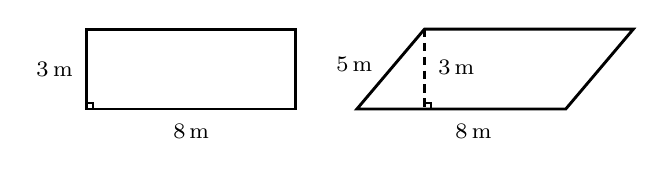
\begin{tikzpicture}[scale=0.39, every node/.style={font=\footnotesize, text=black}]
      \fill[white] (0,0) rectangle (6.8,2.6);
      \draw[black, line width=1.05pt] (0,0) rectangle (6.8,2.6);
      \rightbox[0.20cm]{0,2.6}{0,0}{6.8,0}
      \node[below=2pt] at (3.4,0) {$8\unit{m}$};
      \node[left=1.5pt] at (0,1.3) {$3\unit{m}$};
      \node at (3.5,1.3) {\textbf{ស្រែទី១}};
      \begin{scope}[shift={(8.8,0)}]
        \coordinate (D) at (0,0);
        \coordinate (C) at (6.8,0);
        \coordinate (A) at (2.2,2.6);
        \coordinate (B) at (9.0,2.6);
        \coordinate (F) at (2.2,0);
        \fill[white] (D)--(C)--(B)--(A)--cycle;
        \draw[black, line width=1.05pt] (D)--(C)--(B)--(A)--cycle;
        \draw[black, line width=0.85pt, densely dashed] (A)--(F);
        \rightbox[0.20cm]{A}{F}{C}
        \node[below=2pt] at (3.8,0) {$8\unit{m}$};
        \node[left=1.5pt] at (0.95,1.45) {$5\unit{m}$};
        \node[right=1.5pt] at (2.2,1.35) {$3\unit{m}$};
        \node at (5.8,1.35) {\textbf{ស្រែទី២}};
      \end{scope}
    \end{tikzpicture}
  \end{minipage}
\end{tcolorbox}

% ==================== ផ្នែកទី ២ ៖ E2 - EXPLORE ====================
\secbar{ផ្នែកទី ២ ៖ ការរុករកតាមការប្រៀបធៀបករណីផ្ទុយគ្នា (\enbf{E2 — Contrasting Cases Grid})}{\en{11} នាទី (ពិភាក្សាដៃគូ)}

\textbf{សេចក្ដីណែនាំ៖} ក្រឡាតូចនីមួយៗមានជ្រុង $1$ ឯកតាប្រវែង (ផ្ទៃក្រឡា $1$ ការេឯកតា)។ ចូរសង្កេតរូប \textbf{ករណី A}, \textbf{ករណី B} និង \textbf{ករណី C} រួចបំពេញចន្លោះ៖

\vspace{3pt}
\begin{center}
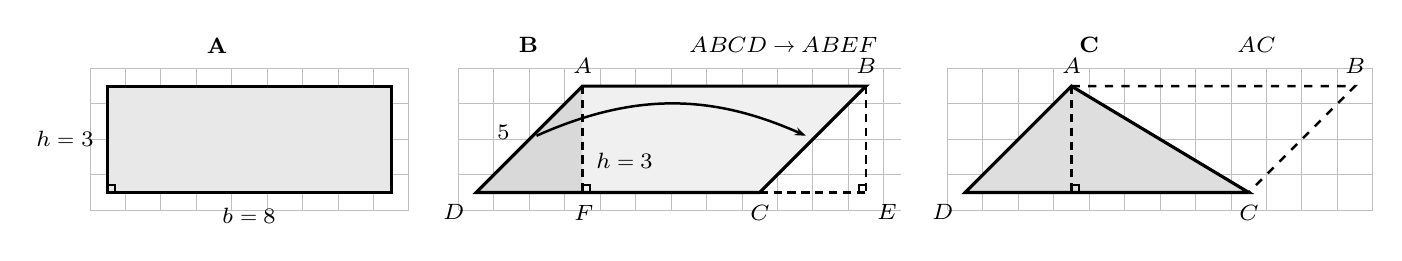
\begin{tikzpicture}[scale=0.45, every node/.style={font=\footnotesize, text=black}]
  % ករណី A
  \begin{scope}[shift={(0,0)}]
    \draw[gray!50, line width=0.35pt] (0,0) grid (9,4);
    \fill[gray!18] (0.5,0.5) rectangle (8.5,3.5);
    \draw[black, line width=1.15pt] (0.5,0.5) rectangle (8.5,3.5);
    \rightbox[0.20cm]{0.5,3.5}{0.5,0.5}{8.5,0.5}
    \node[below=2pt] at (4.5,0.5) {$b = 8$};
    \node[left=1.5pt] at (0.5,2.0) {$h = 3$};
    \node[above=2pt] at (4.5,4.0) {\textbf{ករណី A ៖ ចតុកោណកែងគោល}};
  \end{scope}
  % ករណី B
  \begin{scope}[shift={(10.4,0)}]
    \draw[gray!50, line width=0.35pt] (0,0) grid (12.5,4);
    \coordinate (D) at (0.5,0.5);
    \coordinate (F) at (3.5,0.5);
    \coordinate (C) at (8.5,0.5);
    \coordinate (E) at (11.5,0.5);
    \coordinate (A) at (3.5,3.5);
    \coordinate (B) at (11.5,3.5);
    \fill[gray!30] (D)--(F)--(A)--cycle;
    \fill[gray!12] (F)--(C)--(B)--(A)--cycle;
    \draw[black, line width=1.15pt] (D)--(C)--(B)--(A)--cycle;
    \draw[black, line width=0.95pt, densely dashed] (A)--(F) (B)--(E) (C)--(E);
    \rightbox[0.20cm]{A}{F}{C}
    \rightbox[0.20cm]{B}{E}{C}
    \draw[black, line width=0.9pt, -{Stealth[length=4pt]}, bend left=24] (2.2,2.1) to (9.8,2.1);
    \node[above=1pt] at (A) {$A$};
    \node[above=1pt] at (B) {$B$};
    \node[below left=1pt] at (D) {$D$};
    \node[below=1pt] at (F) {$F$};
    \node[below=1pt] at (C) {$C$};
    \node[below right=1pt] at (E) {$E$};
    \node[left=1pt] at (1.8,2.2) {$5$};
    \node[right=1.5pt] at (3.5,1.4) {$h=3$};
    \node[above=2pt] at (6.25,4.0) {\textbf{ករណី B ៖ បំប្លែងប្រលេឡូក្រាម $ABCD \to ABEF$}};
  \end{scope}
  % ករណី C
  \begin{scope}[shift={(24.2,0)}]
    \draw[gray!50, line width=0.35pt] (0,0) grid (12,4);
    \coordinate (D) at (0.5,0.5);
    \coordinate (F) at (3.5,0.5);
    \coordinate (C) at (8.5,0.5);
    \coordinate (A) at (3.5,3.5);
    \coordinate (B) at (11.5,3.5);
    \fill[gray!26] (A)--(D)--(C)--cycle;
    \draw[black, line width=1.15pt] (A)--(D)--(C)--cycle;
    \draw[black, line width=0.85pt, dashed] (A)--(B)--(C);
    \draw[black, line width=0.9pt, densely dashed] (A)--(F);
    \rightbox[0.20cm]{A}{F}{C}
    \node[above=1pt] at (A) {$A$};
    \node[above=1pt] at (B) {$B$};
    \node[below left=1pt] at (D) {$D$};
    \node[below=1pt] at (C) {$C$};
    \node[above=2pt] at (6.0,4.0) {\textbf{ករណី C ៖ ពុះតាមអង្កត់ទ្រូង $AC$}};
  \end{scope}
\end{tikzpicture}
\end{center}

\vspace{2pt}
\begin{enumerate}[label=\textbf{\arabic*.}, leftmargin=1.5em, itemsep=3pt, topsep=2pt]
  \item \textbf{រាប់ក្រឡាក្នុងករណី A៖} ចតុកោណកែងមានបាត $b = 8$ និងកម្ពស់កែង $h = 3$ មានផ្ទៃក្រឡាសរុបស្មើនឹង \blank{1.8cm} ការេឯកតា។
  \item \textbf{ពិនិត្យករណី B៖} គូសឆ្នូតកាត់ត្រីកោណកែង $\tri{AFD}$ ខាងឆ្វេង រួចរំកិលតាមព្រួញទៅដាក់លើ $\tri{BEC}$ ខាងស្ដាំ៖
  \begin{itemize}[leftmargin=1.3em, itemsep=2pt, topsep=1pt]
    \item ត្រីកោណកែងទាំងពីរមានអ៊ីប៉ូតេនុស $AD = BC =$ \blank{1.3cm} និងជ្រុងមុំកែង $AF = BE =$ \blank{1.3cm} $\Rightarrow \tri{AFD} \cg \tri{BEC}$ តាមករណី \blank{1.6cm}។
    \item ដូចនេះ ប្រលេឡូក្រាម $ABCD$ ប្រែក្លាយជាចតុកោណកែង $ABEF$ ដែលមានបាត $AB =$ \blank{1.3cm} និងទទឹងកែង $AF =$ \blank{1.3cm} មានផ្ទៃក្រឡាសរុបស្មើ \blank{1.6cm} ការេឯកតា។
  \end{itemize}
  \item \textbf{អន្ទាក់ការយល់ច្រឡំ (\en{Misconception Check})៖} ហេតុអ្វីបានជាការគណនា $8 \times 5 = 40$ \textbf{មិនត្រឹមត្រូវ}?\\
  ចម្លើយ៖ ព្រោះអង្កត់ប្រវែង $5$ ជា \blank{3.2cm} ដែលមិន \blank{2.8cm} នឹងបាត $DC$ ឡើយ!
  \item \textbf{ពិនិត្យករណី C (ត្រីកោណ)៖} អង្កត់ទ្រូង $AC$ ចែកប្រលេឡូក្រាមជាត្រីកោណពីរ \blank{2.6cm} ($\tri{ADC} \cg \tri{CBA}$) នាំឱ្យផ្ទៃក្រឡាត្រីកោណ $\tri{ADC}$ ស្មើនឹងពាក់កណ្ដាលផ្ទៃប្រលេឡូក្រាម គឺ $S_{\tri{ADC}} = \dfrac{1}{2} \times$ \blank{1.3cm} $\times$ \blank{1.3cm} $=$ \blank{1.6cm} ការេឯកតា។
\end{enumerate}

% ==================== ផ្នែកទី ៣ ៖ E3 - EXPLAIN ====================
\secbar{ផ្នែកទី ៣ ៖ សំយោគទ្រឹស្ដីបទ រូបមន្ត និងធនាគារហេតុផល (\enbf{E3 — Explain})}{\en{6} នាទី (បំពេញជាមួយគ្រូ)}

\begin{tcolorbox}[
  enhanced, sharp corners, colback=white, colframe=black,
  boxrule=1.0pt, boxsep=2pt, top=4pt, bottom=4pt, left=6pt, right=6pt
]
  $\bullet$ \textbf{ទ្រឹស្ដីបទ (ទំ.១៨៨)៖} ផ្ទៃក្រឡាប្រលេឡូក្រាមដែលមានបាត $b$ និងកម្ពស់កែង $h$ កំណត់ដោយរូបមន្ត៖ $\mathbf{S =}$ \blank{2.5cm} ។\\[3pt]
  $\bullet$ \textbf{សម្រាយបញ្ជាក់សង្ខេប៖} ដោយ $\tri{AFD} \cg \tri{BEC} \implies S_{\tri{AFD}} =$ \blank{1.8cm} ។ គេបាន $S_{ABCD} = S_{ABCF} + S_{\tri{AFD}} = S_{ABCF} +$ \blank{1.8cm} $= S_{ABEF} =$ \blank{1.8cm} ។\\[3pt]
  $\bullet$ \textbf{សម្គាល់ (ផ្ទៃក្រឡាត្រីកោណ)៖} ផ្ទៃក្រឡាត្រីកោណដែលមានបាត $b$ និងកម្ពស់កែង $h$ កំណត់ដោយរូបមន្ត៖ $\mathbf{S_{\tri{}} =}$ \blank{2.8cm} ។\\[4pt]
  \begin{tabular}{|p{4.3cm}|p{4.1cm}|p{4.9cm}|p{3.9cm}|}
    \hline
    \cellcolor{headgray}\centering\textbf{\cnum{1} លក្ខខណ្ឌកែងដាច់ខាត} &
    \cellcolor{headgray}\centering\textbf{\cnum{2} រូបមន្តប្រលេឡូក្រាម} &
    \cellcolor{headgray}\centering\textbf{\cnum{3} សមភាពគូបាត--កម្ពស់} &
    \cellcolor{headgray}\centering\arraybackslash\textbf{\cnum{4} រូបមន្តត្រីកោណ} \\[2pt]
    \hline
    កម្ពស់ $h$ ត្រូវកែងនឹងបាត $b$ ជានិច្ច ($h \perp b$) មិនយកជ្រុងទ្រេតទេ &
    \centering $S = b \times h$ \par (គិតជាឯកតាការេ) &
    ប្រលេឡូក្រាមតែមួយមានគូបាត--កម្ពស់ពីរ៖ $b_1 \times h_1 = b_2 \times h_2$ &
    \centering\arraybackslash $S_{\tri{}} = \dfrac{1}{2} b \times h$ \\[2pt]
    \hline
  \end{tabular}
\end{tcolorbox}

\newpage

% ==================== ទំព័រទី ២ ៖ E4, E5 និងកិច្ចការផ្ទះ ====================
\secbar{ផ្នែកទី ៤ ៖ លំហាត់គំរូបំពេញចន្លោះតាមជំហាន (\enbf{E4 — Faded Worked Examples})}{\en{10} នាទី (សៀវភៅគោល ទំ.១៨៩)}

\begin{tcolorbox}[
  enhanced, sharp corners, colback=white, colframe=black,
  boxrule=0.95pt, boxsep=2pt, top=4pt, bottom=4pt, left=6pt, right=6pt, after skip=5pt
]
  \begin{minipage}[c]{11.8cm}
    \textbf{លំហាត់គំរូទី ១ (ទំ.១៨៩)៖} គេមានប្រលេឡូក្រាម $ABDF$ ដែលមាន $AB = FD = 10\unit{cm}$, $BD = 7\unit{cm}$, $AC = 9\unit{cm}$ ($AC \perp BD$), $AE = x$ ($AE \perp FD$) និង $ED = 8\unit{cm}$ ដូចរូប។\\[2pt]
    \textbf{ជំហានទី ១ \en{[Tracing]}៖} ចូរគូសរង្វង់ព័ទ្ធសញ្ញាមុំកែងទាំងពីរលើរូបខាងស្ដាំ រួចផ្គូផ្គងគូបាត--កម្ពស់៖\\
    \hspace*{0.4cm}-- បាតទី១ $FD = 10\unit{cm}$ ត្រូវនឹងកម្ពស់កែង $AE =$ \blank{1.6cm}\\
    \hspace*{0.4cm}-- បាតទី២ $BD = 7\unit{cm}$ ត្រូវនឹងកម្ពស់កែង $AC =$ \blank{1.6cm}\\[2pt]
    \textbf{ក. គណនាតម្លៃ $x$ (បំពេញចន្លោះតាម \cnum{3})៖}\\
    \hspace*{0.4cm}យើងមាន $FD \times AE = BD \times AC \implies 10 \times x =$ \blank{1.3cm} $\times$ \blank{1.3cm} $=$ \blank{1.5cm}\\
    \hspace*{0.4cm}នាំឱ្យ $x = \dfrac{\blank{1.4cm}}{10} =$ \blank{1.8cm} $\unit{cm}$។\\[2pt]
    \textbf{ខ. រកផ្ទៃក្រឡាត្រីកោណ $AFG$ បើដឹងថា $S_{\tri{AGE}} = 3.15\unit{cm}^2$៖}\\
    \hspace*{0.4cm}-- រកបាត $FE = FD - ED = 10 -$ \blank{1.2cm} $=$ \blank{1.3cm} $\unit{cm}$\\
    \hspace*{0.4cm}-- រកផ្ទៃ $\tri{AFE}$ (កែងត្រង់ $E$)៖ $S_{\tri{AFE}} = \dfrac{1}{2} \times FE \times AE = \dfrac{1}{2} \times$ \blank{1.2cm} $\times$ \blank{1.5cm} $=$ \blank{1.6cm} $\unit{cm}^2$\\
    \hspace*{0.4cm}-- ដូចនេះ $S_{\tri{AFG}} = S_{\tri{AFE}} - S_{\tri{AGE}} =$ \blank{1.5cm} $- 3.15 =$ \blank{1.8cm} $\unit{cm}^2$។
  \end{minipage}\hfill
  \begin{minipage}[c]{6.4cm}
    \centering
    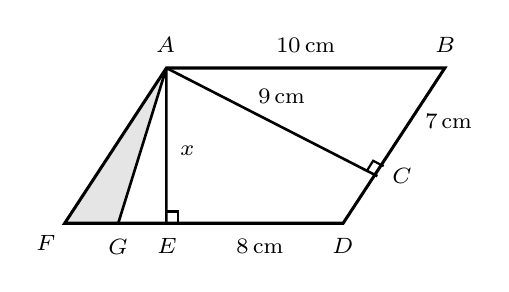
\begin{tikzpicture}[scale=0.68, every node/.style={font=\footnotesize, text=black}]
      \coordinate (F) at (0,0);
      \coordinate (G) at (1.0,0);
      \coordinate (E) at (1.9,0);
      \coordinate (D) at (5.2,0);
      \coordinate (A) at (1.9,2.9);
      \coordinate (B) at (7.1,2.9);
      \coordinate (C) at (5.84,0.88);
      \fill[gray!20] (A)--(F)--(G)--cycle;
      \draw[black, line width=1.1pt] (F)--(D)--(B)--(A)--cycle;
      \draw[black, line width=0.95pt] (A)--(G) (A)--(E) (A)--(C);
      \rightbox[0.22cm]{A}{E}{D}
      \rightbox[0.22cm]{A}{C}{B}
      \node[above=2pt] at (A) {$A$};
      \node[above=2pt] at (B) {$B$};
      \node[below left=1pt] at (F) {$F$};
      \node[below=2pt] at (G) {$G$};
      \node[below=2pt] at (E) {$E$};
      \node[below=2pt] at (D) {$D$};
      \node[right=2pt] at (C) {$C$};
      \node[above=2pt] at (4.5,2.9) {$10\unit{cm}$};
      \node[right=1.5pt] at (1.9,1.35) {$x$};
      \node[above=2pt] at (4.05,1.95) {$9\unit{cm}$};
      \node[right=2pt] at (6.45,1.9) {$7\unit{cm}$};
      \node[below=2pt] at (3.65,0) {$8\unit{cm}$};
    \end{tikzpicture}
  \end{minipage}
\end{tcolorbox}

\begin{tcolorbox}[
  enhanced, sharp corners, colback=panelgray, colframe=black,
  boxrule=0.95pt, boxsep=2pt, top=3.5pt, bottom=3.5pt, left=6pt, right=6pt, after skip=5pt
]
  \begin{minipage}[c]{12.0cm}
    \textbf{លំហាត់គំរូទី ២ (ទំ.១៨៩ — បំពេញជំហានចុងក្រោយដោយខ្លួនឯង)៖}\\
    គណនាផ្ទៃក្រឡាផ្នែកប្រផេះសរុបនៃបន្ទះប្រលេឡូក្រាមទាំង ៣ ក្នុងរូបខាងស្ដាំ៖\\[2pt]
    $\bullet$ បន្ទះប្រផេះនីមួយៗមានបាត $b =$ \blank{1.4cm} $\unit{cm}$ និងកម្ពស់កែងរួម $h =$ \blank{1.4cm} $\unit{cm}$។\\[2pt]
    $\bullet$ $S_{\text{សរុប}} = S_{ABIJ} + S_{CDHI} + S_{DEFG} = 3 \times ($ \blank{1.3cm} $\times$ \blank{1.3cm} $) =$ \blank{2.0cm} $\unit{cm}^2$។\\[2pt]
    $\bullet$ \textbf{សំណួរឆ្លុះបញ្ចាំង៖} ទោះបន្ទះកណ្ដាល $CDHI$ ទ្រេតខ្លាំងជាងគេ ហេតុអ្វីផ្ទៃក្រឡារបស់វាស្មើបន្ទះពីរទៀត? \blank{6.2cm}
  \end{minipage}\hfill
  \begin{minipage}[c]{6.2cm}
    \centering
    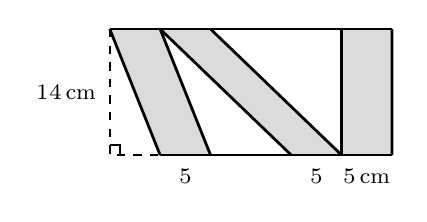
\begin{tikzpicture}[scale=0.64, every node/.style={font=\footnotesize, text=black}]
      \coordinate (A) at (1.0,0);
      \coordinate (B) at (2.0,0);
      \coordinate (C) at (3.6,0);
      \coordinate (D) at (4.6,0);
      \coordinate (E) at (5.6,0);
      \coordinate (J) at (0,2.5);
      \coordinate (I) at (1.0,2.5);
      \coordinate (H) at (2.0,2.5);
      \coordinate (G) at (4.6,2.5);
      \coordinate (F) at (5.6,2.5);
      \fill[gray!28] (A)--(B)--(I)--(J)--cycle;
      \fill[gray!28] (C)--(D)--(H)--(I)--cycle;
      \fill[gray!28] (D)--(E)--(F)--(G)--cycle;
      \draw[black, line width=1.0pt] (J)--(F) (A)--(E);
      \draw[black, line width=1.0pt] (J)--(A) (I)--(B) (I)--(C) (H)--(D) (G)--(D) (F)--(E);
      \draw[black, line width=0.8pt, dashed] (J)--(0,0)--(A);
      \rightbox[0.20cm]{J}{0,0}{A}
      \node[left=1.5pt] at (0,1.25) {$14\unit{cm}$};
      \node[below=1.5pt] at (1.5,0) {$5$};
      \node[below=1.5pt] at (4.1,0) {$5$};
      \node[below=1.5pt] at (5.1,0) {$5\unit{cm}$};
    \end{tikzpicture}
  \end{minipage}
\end{tcolorbox}

% ==================== ផ្នែកទី ៥ ៖ E5 - EVALUATE ====================
\secbar{ផ្នែកទី ៥ ៖ លំហាត់ប្រតិបត្តិ និងវាយតម្លៃរហ័ស (\enbf{E5 — Think-Pair-Check \& Exit Check})}{\en{10} នាទី (ទំ.១៩០)}

\noindent
\begin{minipage}[t]{10.3cm}
  \begin{tcolorbox}[
    enhanced, sharp corners, colback=white, colframe=black,
    boxrule=0.95pt, boxsep=2pt, top=4pt, bottom=4pt, left=5pt, right=5pt, equal height group=e5box
  ]
    \textbf{១. ប្រតិបត្តិ (ទំ.១៩០)៖} $ABCD$ ជាប្រលេឡូក្រាមមាន $AB = 9\unit{cm}$, $AD = 6\unit{cm}$ និង $BK = 8\unit{cm}$ ($BK \perp AD, BH \perp DC$)។
    \begin{center}
      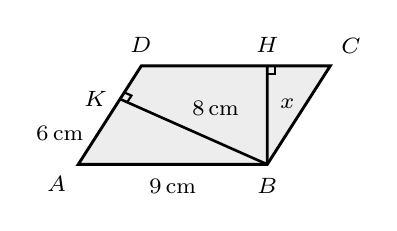
\begin{tikzpicture}[scale=0.50, every node/.style={font=\footnotesize, text=black}]
        \coordinate (A) at (0,0);
        \coordinate (B) at (4.8,0);
        \coordinate (D) at (1.6,2.5);
        \coordinate (C) at (6.4,2.5);
        \coordinate (H) at (4.8,2.5);
        \coordinate (K) at (1.06,1.66);
        \fill[gray!14] (A)--(B)--(C)--(D)--cycle;
        \draw[black, line width=1.05pt] (A)--(B)--(C)--(D)--cycle;
        \draw[black, line width=0.95pt] (B)--(K) (B)--(H);
        \rightbox[0.20cm]{B}{K}{D}
        \rightbox[0.20cm]{B}{H}{C}
        \node[below left=1pt] at (A) {$A$};
        \node[below=1.5pt] at (B) {$B$};
        \node[above right=1pt] at (C) {$C$};
        \node[above=1.5pt] at (D) {$D$};
        \node[above=1.5pt] at (H) {$H$};
        \node[left=1.5pt] at (K) {$K$};
        \node[below=1.5pt] at (2.4,0) {$9\unit{cm}$};
        \node[left=1.5pt] at (0.48,0.8) {$6\unit{cm}$};
        \node[above right=1pt] at (2.6,0.92) {$8\unit{cm}$};
        \node[right=1.2pt] at (4.8,1.55) {$x$};
      \end{tikzpicture}
    \end{center}
    ក. ផ្ទៃក្រឡា $S_{ABCD} =$ \blank{5.8cm}\\[3pt]
    ខ. តម្លៃ $x$ ៖ \blank{6.8cm}\\[3pt]
    \chkbox\ \textit{បានផ្ទៀងផ្ទាត់ជាមួយដៃគូរួចរាល់}
  \end{tcolorbox}
\end{minipage}\hfill
\begin{minipage}[t]{8.4cm}
  \begin{tcolorbox}[
    enhanced, sharp corners, colback=white, colframe=black,
    boxrule=0.95pt, boxsep=2pt, top=4pt, bottom=4pt, left=5pt, right=5pt, equal height group=e5box
  ]
    \textbf{២. តេស្តរហ័ស ៩០ វិនាទី (\en{Exit Check})៖} គណនាផ្ទៃក្រឡាត្រីកោណមុំទាល $\tri{PQR}$ ខាងក្រោម៖
    \begin{center}
      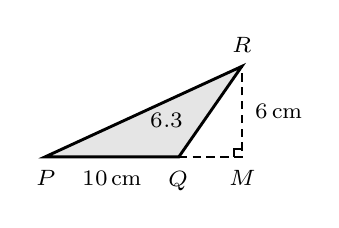
\begin{tikzpicture}[scale=0.50, every node/.style={font=\footnotesize, text=black}]
        \coordinate (P) at (0,0);
        \coordinate (Q) at (3.4,0);
        \coordinate (M) at (5.0,0);
        \coordinate (R) at (5.0,2.3);
        \fill[gray!20] (P)--(Q)--(R)--cycle;
        \draw[black, line width=1.05pt] (P)--(Q)--(R)--cycle;
        \draw[black, line width=0.85pt, densely dashed] (Q)--(M)--(R);
        \rightbox[0.20cm]{R}{M}{Q}
        \node[below=1.5pt] at (P) {$P$};
        \node[below=1.5pt] at (Q) {$Q$};
        \node[below=1.5pt] at (M) {$M$};
        \node[above=1.5pt] at (R) {$R$};
        \node[below=1.5pt] at (1.7,0) {$10\unit{cm}$};
        \node[right=1.5pt] at (5.0,1.15) {$6\unit{cm}$};
        \node[left=2pt] at (3.9,0.92) {$6.3$};
      \end{tikzpicture}
    \end{center}
    គូសធីកចម្លើយត្រឹមត្រូវតែ ១៖\\
    \chkbox\ \textbf{A.} $60\unit{cm}^2$ \hspace{0.9cm} \chkbox\ \textbf{B.} $30\unit{cm}^2$\\[2pt]
    \chkbox\ \textbf{C.} $31.5\unit{cm}^2$ \hspace{0.65cm} \chkbox\ \textbf{D.} $63\unit{cm}^2$\\[2pt]
    \textbf{បិទបេសកកម្ម E1៖} $S_{\text{ស្រែទី២}} =$ \blank{2.0cm} $\unit{m}^2$។
  \end{tcolorbox}
\end{minipage}

% ==================== កិច្ចការផ្ទះ (ជំហានទី ៥) ====================
\vspace{4pt}
\begin{tcolorbox}[
  enhanced, sharp corners, colback=panelgray, colframe=black,
  boxrule=1.0pt, boxsep=2pt, top=3.5pt, bottom=3.5pt, left=6pt, right=6pt
]
  {\muol\fontsize{9.0pt}{13pt}\selectfont កិច្ចការផ្ទះ (សៀវភៅសិក្សាគោល ទំព័រ ១៩៤ — ធ្វើដាក់ក្នុងសៀវភៅលំហាត់សម្រាប់ម៉ោងក្រោយ)}\\[2pt]
  $\bullet$ \textbf{លំហាត់ទី ១ (ទំ.១៩៤)៖} បំពេញតារាងប្រលេឡូក្រាម៖ (ក) បាត $12\unit{cm}$, កម្ពស់ $7\unit{cm} \Rightarrow S = ?$ \;\vert\; (ខ) កម្ពស់ $6\unit{cm}, S = 42\unit{cm}^2 \Rightarrow b = ?$ \;\vert\; (គ) បាត $7.8\unit{cm}, S = 42.9\unit{cm}^2 \Rightarrow h = ?$។\\
  $\bullet$ \textbf{លំហាត់ទី ២ រូបទី១ (ទំ.១៩៤)៖} ប្រលេឡូក្រាម $SRQP$ មានបាត $PQ = SR = 28\unit{cm}$, កម្ពស់ $SH = 7\unit{cm}$, ជ្រុង $RQ = SP = 8\unit{cm}$ និងកម្ពស់ $PR = x$ ($PR \perp RQ$)។ គណនាតម្លៃ $x$។ \textit{(អានមុន៖ ចំណុច ២. ផ្ទៃក្រឡាចតុកោណស្មើ ទំ.១៩០--១៩១)}
\end{tcolorbox}

\end{document}
